\documentclass[11pt,a4paper]{article}
\usepackage[T1]{fontenc}
\usepackage[utf8]{inputenc}
\usepackage{lmodern}
\usepackage[margin=25mm,headheight=14pt]{geometry}
\usepackage{microtype}
\usepackage{amsmath,amssymb}
\usepackage{booktabs,tabularx,longtable,array}
\usepackage{enumitem}
\usepackage{needspace}
\usepackage{listings}
\usepackage{tikz}
\usetikzlibrary{arrows.meta,positioning}
\usepackage{fancyhdr}
\usepackage{xurl}
\usepackage[hidelinks,pdfusetitle]{hyperref}
\setlength{\parindent}{0pt}
\setlength{\parskip}{6pt}
\setlength{\emergencystretch}{2em}
\setlist{nosep,leftmargin=1.5em,topsep=4pt}
\setcounter{tocdepth}{2}
\renewcommand{\arraystretch}{1.15}
\setlength{\tabcolsep}{4pt}
\newcolumntype{Y}{>{\raggedright\arraybackslash}X}
\newcolumntype{P}[1]{>{\raggedright\arraybackslash}p{#1}}
\newcommand{\code}[1]{\nolinkurl{#1}}
\newcommand{\file}[1]{\path{#1}}
\lstset{basicstyle=\ttfamily\footnotesize,columns=fullflexible,
  keepspaces=true,breaklines=true,showstringspaces=false,
  frame=single,framerule=0.2pt,framesep=5pt,
  aboveskip=8pt,belowskip=8pt,upquote=true}
\pagestyle{fancy}
\fancyhf{}
\fancyhead[L]{\small ABOX2TBOX}
\fancyhead[R]{\small Project guide}
\fancyfoot[C]{\thepage}
\renewcommand{\headrulewidth}{0.2pt}
\title{ABOX2TBOX\\[5pt]\large Purpose, implementation, operation, and alternatives}
\author{Project documentation}
\date{19 October 2026\\[3pt]\small Implementation snapshot: \texttt{7a98c41} / pipeline v3.1}

\hypersetup{pdftitle={ABOX2TBOX: Project Guide},pdfauthor={Project documentation}}

\begin{document}
\maketitle
\thispagestyle{plain}

\begin{abstract}
ABOX2TBOX is an experimental Python pipeline that turns patterns in RDF instance
assertions into proposed OWL schema axioms. It combines RDFLib, in-memory SQL,
statistical candidate mining, optional structured model decisions, graph repair,
and HermiT reasoning. Its output is a candidate ontology for assessment, not an
automatically established account of a domain.

This guide explains what the project does, why its components exist, how the
notebook runs, where its implementation lives, and when another approach is a
better fit. It documents the current single-model design and the limits of its
validation and evaluation. Comparisons are engineering judgments grounded in
tool capabilities; they are not claims of measured superiority.
\end{abstract}

\textbf{The central distinction.} RDFLib manages RDF; the project builds an
induction workflow on top of it. A model may help judge a candidate. A reasoner
checks the consequences of accepted axioms. These are separate responsibilities.

\textbf{Reading routes.} For the idea, read Sections~\ref{sec:purpose}--\ref{sec:architecture}.
For execution, start at Section~\ref{sec:operation}. For choosing an approach,
read Sections~\ref{sec:alternatives} and~\ref{sec:recommendation}. For research
claims, read Sections~\ref{sec:evaluation} and~\ref{sec:limits} first.

\newpage
\tableofcontents
\newpage

\section{Purpose and scope}\label{sec:purpose}

\subsection{The problem the project addresses}
An RDF dataset may identify people, sensors, transactions, crops, or other
entities, yet provide only fragments of their conceptual structure. There may be
no useful class hierarchy, many entities may be untyped, and relationships may
lack an explicit domain or range. Writing the missing schema by hand can require
considerable inspection.

The project proposes a first draft from recurring evidence. Shared property
signatures suggest groups of entities; repeated type co-membership suggests
possible subclass relations; repeated paths suggest role rules. An optional
model judges whether some patterns have a plausible universal interpretation.
The resulting OWL graph can then support expert discussion and further testing.

Useful settings include exploratory ontology construction, comparing multiple
schemas inferred from the same data, and inspecting which regularities a domain
expert might formalize. The project is less appropriate when the schema is
already authoritative, when only data-format validation is needed, or when a
production service requires a measured latency and memory envelope.

\subsection{ABox, TBox, and a running example}
An \emph{ABox} contains assertions about individuals. A \emph{TBox} describes
classes and relationships between classes. OWL gives such statements a logical
interpretation and supports deriving consequences~\cite{owl-primer}.

For example, these instance facts could appear in a Turtle input:
\begin{lstlisting}
@prefix ex: <https://example.org/> .
ex:alice a ex:GraduateStudent, ex:Student ;
         ex:enrolledAt ex:university1 .
ex:bob   a ex:GraduateStudent, ex:Student ;
         ex:enrolledAt ex:university1 .
\end{lstlisting}
A candidate schema statement is:
\begin{lstlisting}
@prefix rdfs: <http://www.w3.org/2000/01/rdf-schema#> .
ex:GraduateStudent rdfs:subClassOf ex:Student .
\end{lstlisting}
The two observations motivate a question; they do not establish a universal
rule. This tiny illustration is also below the current offline minimum support
of five. The notebook does not admit it merely because the example looks
reasonable.

\subsection{The semantic trap: absence is not a negative label}
OWL uses an open-world interpretation: an unrecorded fact need not be false.
Distinct identifiers also need not denote distinct individuals~\cite{owl-primer}.
Consequently, a lack of shared observed members does not prove disjointness.
An observed single value per subject does not establish that the property can
never have two values. A functional property can also imply equality of fillers
rather than produce a database-style duplicate-value error.

The pipeline therefore separates observed support, model judgment, and logical
validation. Even after all three, expert assessment and independent evaluation
remain necessary before promoting a candidate to a domain commitment.

\section{Architecture and rationale}\label{sec:architecture}

\begin{figure}[htbp]
\centering
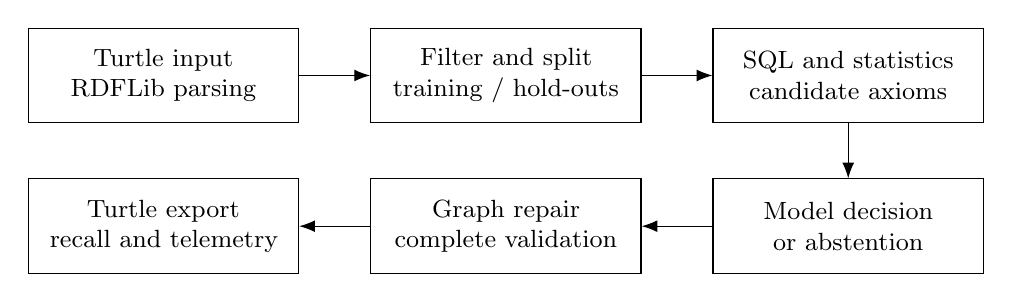
\begin{tikzpicture}[node distance=7mm and 9mm,
 box/.style={draw,rectangle,align=center,font=\small,minimum height=12mm,text width=32mm},
 arr/.style={-{Latex[length=2mm]},thin}]
\node[box] (input) {Turtle input\\RDFLib parsing};
\node[box,right=of input] (split) {Filter and split\\training / hold-outs};
\node[box,right=of split] (mine) {SQL and statistics\\candidate axioms};
\node[box,below=of mine] (decide) {Model decision\\or abstention};
\node[box,left=of decide] (repair) {Graph repair\\complete validation};
\node[box,left=of repair] (export) {Turtle export\\recall and telemetry};
\draw[arr] (input)--(split);
\draw[arr] (split)--(mine);
\draw[arr] (mine)--(decide);
\draw[arr] (decide)--(repair);
\draw[arr] (repair)--(export);
\end{tikzpicture}
\caption{The implemented workflow. Hold-out labels are consulted only in evaluation.
Independent calibration labels are also loaded after induction and export.}
\end{figure}

\begin{tabularx}{\textwidth}{@{}P{28mm}YY@{}}
\toprule
Component & Responsibility & Why it exists here \\
\midrule
RDFLib & Parse, represent, query, construct, and serialize RDF. & Preserves the RDF graph model and provides interoperable input/output. \\
SQLite & Store an indexed training-triple projection in memory. & Makes repeated subject/predicate lookups convenient. It does not provide persistence in this configuration. \\
Python statistics & Compute signatures, support, overlap, and candidate scores. & Supplies inspectable evidence before a model is asked a question. \\
Decision transport & Submit structured questions and validate numeric responses. & Supports optional semantic judgment, bounded attempts, and abstention. \\
NetworkX & Represent the taxonomy and repair graph structure. & Supports cycle detection, reachability, and transitive reduction. \\
Owlready2 / HermiT & Load an OWL serialization and check reasoning outcomes. & Checks named-class coherence and consistency with the retained training assertions. \\
Matplotlib & Draw descriptive diagnostics. & Makes the output easier to inspect; the plot is not a validation certificate. \\
\bottomrule
\end{tabularx}

RDFLib's central abstraction is an RDF graph with triple-oriented operations~\cite{rdflib}.
The current approach already uses that abstraction. Asking whether this project
is better than RDFLib alone compares a workflow with one of its components.
The meaningful comparison is with a deterministic induction workflow implemented
using RDFLib and explicit rules.

SQLite and RDFLib hold overlapping representations, which simplifies inspection
but increases memory use. NetworkX operates on a schema graph, not on the full
RDF semantics. HermiT is accessed through Owlready2's reasoning integration and
requires Java~\cite{owlready}. None of these libraries independently supplies the
whole induction method.

\Needspace{8\baselineskip}
\section{Repository map: where things live}\label{sec:map}

\begin{longtable}{@{}P{58mm}P{99mm}@{}}
\toprule
Path & Purpose \\
\midrule
\endfirsthead
\toprule Path & Purpose \\ \midrule
\endhead
\file{abox2tbox.ipynb} & Main entry point: configuration, preprocessing, mining, adjudication, graph construction, and evaluation. Execute in order from a fresh kernel. \\
\file{pipeline_support.py} & Reusable transport, numeric validation, class closure, role repair, export validation, recovery, and calibration functions. \\
\file{build_notebook.py} & A generator containing synchronized, output-free cell sources. Running it overwrites the notebook. \\
\file{requirements.txt} & Pinned Python runtime dependencies. Notebook and test tools are separate installation needs. \\
\file{input/} & Turtle datasets. Filenames are case-sensitive; \file{ABox.ttl}, \file{ABOX.ttl}, and \file{agriAbox.ttl} are different paths. \\
\file{output/TBox.ttl} & Default validated schema export. It may be from an earlier run; inspect execution status and timestamps. \\
\file{output/telemetry_diagnostics.png} & Default diagnostics image. It is generated after schema export and is not committed atomically with it. \\
\file{test_complete_v3.py} & Focused regression tests against the notebook and support code, including mocked transport behavior and failure cases. \\
\file{test_pipeline.py} & Offline end-to-end checks on the baseline dataset, with temporary outputs. \\
\file{test_cross_domain.py} & Offline checks on the baseline, e-commerce, hospital, enterprise, and banking fixtures. \\
\file{README.md} & Short installation, operation, and interpretation guide. \\
\file{docs/project-guide.tex} & This document's editable source. \\
\file{docs/project-guide.pdf} & Compiled reading copy; the remaining LaTeX files in this directory are retained build residuals. \\
\bottomrule
\end{longtable}

The baseline harness still uses the historical label ``University Baseline.''
The supplied \file{input/ABox.ttl} examined for this implementation contains
smart-city class identifiers. Verify a dataset's actual content before attaching
a domain interpretation to its filename or harness label.

\section{How the pipeline works}\label{sec:workflow}

\subsection{Parse, filter, and construct the training graph}
The notebook parses Turtle using RDFLib. If blank nodes occur, it canonicalizes
the graph to stabilize their identifiers. It removes subjects declared as schema
or metadata entities, declared annotation properties, and predicates in the
RDF/RDFS/OWL/XSD metadata namespaces, with a special allowance for retained domain
\code{rdf:type} assertions.

This preprocessing defines the induction view. Validation later uses that
retained view, not the entire raw input. For example, filtering can remove
\code{owl:sameAs} and existing schema assertions. A successful check therefore
must not be described as validation against every statement in the source file.
A dataset containing important existing semantics needs an explicit preservation
or import policy before the workflow is used as an integration system.

\subsection{Deterministic hold-outs}
With seed 42, the notebook samples 20\% of entities that have at least two
retained types and removes one randomly chosen type from each sampled entity.
Separately, it removes 15\% of retained non-literal role triples. Counts are
rounded; small datasets can have zero hold-outs. Literal assertions are not
withheld by this procedure.

Sorting and canonicalization make the split reproducible for unchanged data and
code. The retained graph becomes \code{training_graph}; the original graph is
removed from later mining state. Held-out assertions remain available for
recovery evaluation, not for candidate selection or repair.

Type recall is consequently conditional on the multi-typed population. It does
not estimate performance on every entity, on wholly unseen individuals, or on
classes absent from training. Every normal run exports a schema learned from the
training subset. There is currently no separate automatic full-data retraining
pass after evaluation.

\subsection{Indexed projection and entity grouping}
Training triples are inserted into an in-memory SQLite table with subject,
predicate, object, literal status, and datatype columns. Literals use N3 strings,
retaining datatype and language identity for counting. Composite indexes support
subject/predicate and predicate/object access.

Untyped subjects are grouped by outgoing and incoming predicate signatures.
Micro-clusters with compatible incoming signatures can merge when their outgoing
weighted Jaccard similarity reaches 0.65. Predicate weights are based on
\[
  w(p)=\log\!\left(1+\frac{N}{df(p)}\right),\qquad
  J_w(A,B)=\frac{\sum_{p\in A\cap B}w(p)}{\sum_{p\in A\cup B}w(p)}.
\]
Here $N$ is the retained subject count and $df(p)$ counts subjects using $p$.
A merged core predicate occurs in at least half of the merged entities.

These clusters are provisional structural groupings. Similar records can reflect
a shared ingestion template rather than a natural kind. Object-only resources
with no outgoing subject occurrence are not automatically handled as a complete
entity population by this grouping stage.

\subsection{Names and class candidates}
The dominant namespace is estimated from retained classes, predicates, and
subjects after standard vocabulary filtering. New class names are formed
deterministically from property-name tokens. A model may choose among those
names. Alignment to an existing class requires a close lexical match, matching
observed predicates, and explicit model confirmation.

The generated class descriptions identify a provisional signature grouping.
The competency-style question is a template derived from the signature; it is
not independently elicited from domain stakeholders. Namespace frequency can
favor a broad vocabulary over the intended application namespace, so inspect
all newly minted identifiers.

\subsection{Taxonomic candidate mining}
For observed class instance sets $I_C$ and $I_D$, the notebook computes
\[
  \widehat{s}(C,D)=\frac{|I_C\cap I_D|}{|I_C|},\qquad
  J(C,D)=\frac{|I_C\cap I_D|}{|I_C\cup I_D|}.
\]
The first is observed coverage of $C$ by $D$, not an independently calibrated
probability that $C\sqsubseteq D$. A Wilson lower bound summarizes uncertainty in
sample coverage; the configured $z$ is 1.28. Candidate collection uses a maximum
directional coverage of at least 0.15 or Jaccard of at least 0.35.

For some non-overlapping pairs involving induced classes, predicate-intent
containment provides another candidate route. If $S_C$ and $S_D$ are property
signatures, the structural evidence toward $C\sqsubseteq D$ uses
$|S_C\cap S_D|/|S_D|$: a more specialized description should cover its proposed
parent's predicates. Such evidence proposes a question; it does not prove that
property occurrence defines class membership. The implementation does not build
a complete formal-concept lattice.

Candidates are sorted by observed overlap and identifiers, then capped by
\code{MAX_DECISION_PAIRS}. The pairwise mining loops run before this cap, so the
cap does not bound the cost of discovering candidates.

\subsection{Role rules and class restrictions}
The notebook considers selected role-rule templates:
\begin{align*}
 p(x,y)&\Rightarrow q(x,y) &&\text{(subproperty)},\\
 p(x,y)&\Rightarrow q(y,x) &&\text{(inverse candidate)},\\
 p_1(x,z)\wedge p_2(z,y)&\Rightarrow p_3(x,y) &&\text{(two-hop chain)}.
\end{align*}
It uses support, head coverage, and partial-completeness-style confidence.
This is a limited template miner inspired by the same general concern about
incomplete observations that motivates AMIE; it does not invoke the AMIE
implementation~\cite{amie}. Minimum supporting counts and additional confidence
thresholds apply before a proposal reaches model confirmation.

For local restrictions, positive instances are the observed members of a class
and the remaining observed domain instances act as a comparison population.
This population is an operational negative set, not a guarantee of semantic
non-membership. Coverage scores can therefore be affected by missing types.
The one-step heuristic is
\[
 \phi=q_{\mathrm{ref}}+\lambda(q_{\mathrm{ref}}-q_{\mathrm{parent}})
             -\beta\ell,
 \quad q_{\mathrm{parent}}=0.5,\quad \ell=3,
\]
with $q_{\mathrm{ref}}$ computed from observed F1, $\lambda=0.20$, and
$\beta=0.03$. Existential candidates require score at least 0.70 and positive
coverage at least 0.50. Universal candidates use observed filler purity at least
0.95 and at least three matching edges. This is not a complete CELOE search.

Mixed literal/object use of a single predicate causes an explicit error, because
the exporter cannot simply declare that predicate as both an OWL object and
datatype property. Normalize the data or define an explicit mapping policy.

\subsection{Adjudication and abstention}
Taxonomic model decisions choose one of two subclass directions, equivalence,
or insufficient evidence. Admission requires a valid four-choice probability
distribution, chosen probability at least 0.70, confidence at least 0.55, and
necessity score at least 2.5 out of 3. These are model-reported values.

If no answer is available, offline subclass admission requires exact observed
inclusion, support of at least five, Wilson lower bound at least 0.70, and a
strictly smaller observed child class. The result is marked
\code{empirical_inclusion}. Equal observed extensions do not become equivalence.
Signature-only candidates do not become offline subclass axioms.

Disjointness, role characteristics, subproperties, inverses, chains, local
restrictions, and domain/range axioms require explicit confirmation: validity
at least 0.90 and necessity at least 2.5. Property characteristics also require
support and the corresponding observed evidence gate. A lack of observed
compositions yields zero transitivity evidence rather than automatic acceptance.
The model is still a fallible judge of universality.

\subsection{Repair and complete-export validation}
The taxonomy is a directed graph with edges from subclass to superclass. Greedy
repair removes a weak edge from a detected cycle until the graph is acyclic.
Transitive reduction removes redundant asserted edges while preserving reachable
named-class relationships. This procedure is not weighted MaxSAT and makes no
global optimality claim.

Equivalences participate in the closure used to detect disjointness conflicts.
Role repair propagates non-simplicity through property relationships and rejects
chains that violate its conservative dependency-order test. Some legal recursive
chains may be rejected. OWL 2 DL imposes global restrictions beyond ordinary RDF
syntax, including restrictions on the use of non-simple roles~\cite{owl-syntax}.
The custom checks are not a comprehensive external OWL profile validator.

After every accepted axiom has been added, the complete Turtle serialization is
parsed back and checked by HermiT. First, named classes must be satisfiable in the
TBox; then the TBox is checked with retained training assertions and induced
memberships. Missing Java, reasoning errors, inconsistency, and detected
unsatisfiable classes stop the export. The reasoner does not establish empirical
truth or whether an induced concept is useful.

Only after validation does the notebook atomically replace the TBox file. The
schema remains a logical hypothesis even after this gate: empirical inclusion
can be universally false without causing a contradiction in the available data.

\section{Decision AI and Generative AI}\label{sec:ai}

The current code has one active model setting, \code{MODEL_DECISION}, whose
default value is \code{clef-flash:latest}. It uses that model to select names and
judge proposed axioms. There is no active \code{MODEL_GENERATIVE} setting and no
separate Qwen text-generation stage.

\begin{tabularx}{\textwidth}{@{}P{35mm}YY@{}}
\toprule
Role & Current behavior & Possible future behavior \\
\midrule
Candidate generation & Statistical templates and deterministic names. & A generative model could propose richer names, definitions, competency questions, or axiom candidates. \\
Decision & One configured model returns structured choices and scores. & A distinct judge could assess proposals with independently supplied evidence. \\
Validation & Deterministic structural checks and HermiT. & Additional OWL profile, SHACL, or domain-specific checks could be introduced. \\
\bottomrule
\end{tabularx}

The terms \emph{Decision AI} and \emph{Generative AI} describe roles in this
architecture, not necessarily disjoint kinds of underlying models. The chat
fallback generates JSON text to perform a decision task. That does not create
a separate free-form ontology-generation phase.

\subsection{The two transport routes}
The transport first probes the configured server's \code{/v1/systemone} route,
expecting an \code{answers} object. This is a project-specific contract; a
standard Ollama installation should not be assumed to implement it.

If the probe fails, the transport tries \code{/api/chat} with JSON output,
streaming disabled, temperature zero, and seed 42. Ollama documents this chat
endpoint and structured-output options~\cite{ollama}. Both routes use the same
configured decision model. If neither succeeds, the run uses statistical mode.
A successful connection is not proof that every later candidate receives a
usable decision.

\subsection{Would a two-model design be better?}
A generator could offer names and definitions beyond the current deterministic
vocabulary. It could also introduce unsupported ideas or steer the judge toward
its own wording. A separate judge does not guarantee independent errors.
An engineering decision to add generation should therefore be based on an
ablation study with reviewed axioms, runtime, and cost, rather than the number
of AI stages. Section~\ref{sec:experiment} gives a comparison plan.

\section{Installation and operation}\label{sec:operation}

\subsection{Start from the repository root}
Use a compatible Python environment, Java for HermiT, and a notebook interface.
The runtime pins in \file{requirements.txt} do not themselves install Jupyter
or pytest. One possible setup is:
\begin{lstlisting}
python3 -m venv .venv
. .venv/bin/activate
python -m pip install -r requirements.txt
python -m pip install jupyterlab pytest
java -version
\end{lstlisting}
The current pins are RDFLib 7.6.0, NetworkX 3.7, Matplotlib 3.11.2, NumPy 2.5.4,
Ollama 0.6.3, and Owlready2 0.51. They record the project's current environment;
they are not a promise of compatibility with every Python or operating-system
version. The transport currently uses Python's HTTP facilities; the installed
Ollama package is not the mechanism issuing these decision requests.

\subsection{Run offline first}
\begin{lstlisting}
export USE_LLM=false
export ABOX_INPUT_PATH="$PWD/input/ABox.ttl"
export TBOX_OUTPUT_PATH="$PWD/output/TBox.ttl"
export TELEMETRY_PLOT_PATH="$PWD/output/telemetry_diagnostics.png"
jupyter lab abox2tbox.ipynb
\end{lstlisting}
Restart the kernel and run all cells in order. The default working directory
controls relative paths and discovery of \file{pipeline_support.py}. The
notebook's dependency cell is a commented installation hint; it does not run pip
on every execution.

The notebook otherwise defaults to \file{input/agriAbox.ttl}. That file was a
local untracked dataset at the documented snapshot and was not included in the
implementation push. A fresh clone should explicitly choose a bundled input or
provide the agricultural file at the expected path.

Offline mode can finish with few expressive axioms and low recall. That is an
observable property of the conservative rules, not evidence that an AI endpoint
was silently used. The schema export contains class declarations and accepted
hypotheses; it is not a new copy of the full input ABox.

\subsection{Enable model-assisted decisions}
\begin{lstlisting}
export USE_LLM=true
export OLLAMA_BASE_URL=http://localhost:11434
export MODEL_DECISION=clef-flash:latest
export LLM_TIMEOUT_S=20
jupyter lab abox2tbox.ipynb
\end{lstlisting}
Ensure the configured model is actually available and supports the required
response behavior. The repository's retained endpoint default is a private
network address, \code{http://100.75.221.29:11434}; it is not a portable service
provided with the project. Only the configured endpoint is contacted.

Candidate identifiers and some counts or properties are sent to the server.
Choose the endpoint with that data movement in mind. Native and chat decisions
may differ, and model or server changes can alter results even when the Python
seed is unchanged.

\subsection{Run the tests}
\begin{lstlisting}
python -m pytest test_complete_v3.py test_pipeline.py \
  test_cross_domain.py -q
\end{lstlisting}
The documented implementation check completed with 73 passing tests, including
the five bundled domain fixtures. Tests use temporary output paths, restore
changed environment variables, and avoid live model requests. Mocked transport
checks cover native/chat behavior, size gates, limits, malformed values, errors,
and circuit breaking. Reasoner tests include intentionally invalid ontologies.

This is evidence about checked behavior. It is not a benchmark proving that AI
improves ontology quality. The live decision server and the complete 50~MB
agricultural input were not verified by that test result.

\section{Configuration: what can actually be changed}\label{sec:config}

\begin{longtable}{@{}P{54mm}P{35mm}P{65mm}@{}}
\toprule
Environment variable & Default & Effect \\
\midrule
\endfirsthead
\toprule Environment variable & Default & Effect \\ \midrule
\endhead
\code{USE_LLM} & \code{true} & Enables transport probing; false makes the run offline. \\
\code{OLLAMA_BASE_URL} & Private server & Server base URL, including port; see Section~\ref{sec:operation}. \\
\code{MODEL_DECISION} & \code{clef-flash:latest} & Model used for naming decisions and axiom adjudication. \\
\code{LLM_TIMEOUT_S} & 20.0 & Timeout passed to individual HTTP calls, not a whole-run deadline. \\
\code{MAX_DECISION_PAIRS} & 1000 & Caps taxonomic candidates after mining and bounds shared decision attempts across stages. \\
\code{MAX_LLM_PAIRS} & 1000 & Caps model decision attempts; readiness probes are separate. \\
\code{MAX_PAYLOAD_TOKENS} & 1500 & Gates a byte-based preflight estimate; also checks reported input usage after a response. \\
\code{LLM_MAX_CONSECUTIVE_ERRORS} & 3 & Opens the shared circuit after consecutive request failures. \\
\code{SYSTEMONE_BATCH_SIZE} & 16 & Validated legacy setting. The current transport sends one candidate per call; changing it does not enable batching. \\
\code{ABOX_INPUT_PATH} & Local agriculture file & Turtle input; override it for bundled fixtures. \\
\code{TBOX_OUTPUT_PATH} & \file{output/TBox.ttl} & Validated schema destination. \\
\code{TELEMETRY_PLOT_PATH} & Diagnostics PNG & Plot destination, resolved from the working directory by default. \\
\code{CALIBRATION_LABELS_PATH} & Unset & Optional independent directed binary labels, loaded after induction/export. \\
\bottomrule
\end{longtable}

Other settings, such as hold-out fractions, Jaccard thresholds, Wilson $z$, and
restriction scoring coefficients, are currently values in the notebook's
configuration dictionary. Setting a similarly named shell variable does not
automatically override them. Some historical keys remain but no longer control
the active gates: for example, general axiom confirmation uses its explicit 0.90
and 2.5 thresholds, and taxonomic necessity uses 2.5 rather than
\code{THETA_SCORE}. Trace the actual call site before tuning a parameter.

\subsection{Budget semantics and audit interpretation}
Preflight sizing uses serialized UTF-8 bytes plus a reserve of 128, recorded as
\code{estimated_input_tokens}. This name is historical: it is an estimate, not
an exact tokenizer measurement. Server prompt framing and tokenization can differ.
Oversized requests abstain before sending; a reported input-token overrun disables
further calls after the overrun is observed.

Audit records include stage, endpoint, model, timestamp, status, estimated size,
and reported input usage if supplied. Reported usage is \code{None} when unknown.
No fictitious readiness call is recorded in offline mode. Shared attempt budgets
are consumed in pipeline order, including naming; later stages may receive no
model budget. Some limit-based returns happen before an audit event is created,
so the audit is a request log, not a full ledger of every rejected candidate.

\section{Artifacts, provenance, and guarantees}\label{sec:artifacts}

The principal deliverable is a Turtle ontology. It can contain named classes,
subclass and equivalence axioms, disjointness, property declarations and
characteristics, domains and object ranges, local restrictions, subproperties,
inverses, and property chains. Which families occur depends on the data and
adjudication outcome.

For subclass axioms, OWL axiom annotations distinguish empirical support from
model decision probability and record confidence, support count, mining mode,
and source. Pipeline attribution uses an IRI for the pipeline agent. PROV-O
provides a standard vocabulary for provenance relationships~\cite{prov}.
The current metadata does not preserve a complete reproducible model execution:
there is no automatically persisted manifest of dataset hashes, model digests,
prompts, responses, every rejection, and all configuration values. Expressive
axiom families do not all carry the same detailed per-axiom source annotations.

\begin{tabularx}{\textwidth}{@{}YY@{}}
\toprule
What a successful export supports & What it does not establish \\
\midrule
The serialized file parsed back as Turtle. & That the chosen vocabulary matches the intended domain. \\
Selected structural and role checks passed. & Comprehensive OWL 2 DL profile certification for arbitrary input. \\
HermiT found no forbidden outcome in the constructed TBox checks. & That every axiom is true outside the retained training data. \\
The constructed TBox is consistent with the retained training ABox. & Consistency with every raw assertion, external dataset, or future observation. \\
The TBox destination was replaced only after validation. & An atomic transaction over the TBox, plot, logs, and evaluation results. \\
\bottomrule
\end{tabularx}

A failure in plotting or reading calibration labels can occur after a new TBox
has already been written. Conversely, a failed pre-export validation leaves the
previous TBox in place. Record the run status; file existence alone is ambiguous.
Audit variables and numeric metrics are mainly kernel state and printed output,
so save them explicitly if a run must be compared later.

\section{Evaluation: what the numbers mean}\label{sec:evaluation}

\subsection{Positive hold-out recall}
For held-out type assertions $H_t$ and recovered type assertions $R_t$,
\[
  \mathrm{recall}_{t}=\frac{|H_t\cap R_t|}{|H_t|}.
\]
The role metric uses the same construction with held-out named edges. If a
hold-out set is empty, the corresponding result is unavailable. Precision and
F1 are \code{None} because the dataset does not supply independently labeled
negative assertions. Counting every unobserved fact as false would contradict
the intended incomplete-data setting.

Recovery applies a supported rule fragment: named-class subclass/equivalence
closure, domains/ranges, subproperties, inverses, chains, symmetry, reflexivity,
and transitivity. It does not perform full OWL entailment, equality reasoning,
existential witness recovery, or restriction-based type inference. Recall
therefore measures the behavior of that fragment, not all inferences HermiT
could potentially support.

\subsection{Calibration against independent labels}
Provide a JSON file of directed subclass labels to enable calibration:
\begin{lstlisting}
[
  {"sub": "https://example.org/Student",
   "super": "https://example.org/Person", "label": 1},
  {"sub": "https://example.org/Person",
   "super": "https://example.org/Student", "label": 0}
]
\end{lstlisting}
\begin{lstlisting}
export CALIBRATION_LABELS_PATH="$PWD/labels.json"
\end{lstlisting}
Labels must be unique directed pairs with binary values. They should be reviewed
independently and account for indirect subclass entailment. A negative label
means the proposed universal axiom is rejected under the evaluation protocol;
it does not require that the two classes be disjoint.

Only pairs with both an available model prediction and a supplied label are
scored. Thus the calibration count is also a coverage indicator, not the size of
the entire gold set. Directed subclass probability combines the chosen direction
with equivalence probability mass. Offline overlap statistics are not substituted
for model probabilities.

For $n$ scored predictions, the implemented Brier score is
\[
 \mathrm{Brier}=\frac{1}{n}\sum_{i=1}^{n}(p_i-y_i)^2.
\]
With nonempty bins $B_m$, expected calibration error is
\[
 \mathrm{ECE}=\sum_m\frac{|B_m|}{n}
   \left|\frac{\sum_{i\in B_m}p_i}{|B_m|}
              -\frac{\sum_{i\in B_m}y_i}{|B_m|}\right|.
\]
There are ten fixed-width bins, including probability 1.0 in the final bin;
empty bins are omitted. No overlapping independent labels means unavailable
metrics. ECE depends on binning and label composition, so comparisons require
the same evaluation population and coverage reporting.

\subsection{Descriptive metrics are not accuracy}
The following definitions describe the current code rather than a claim of
universal metric standardization. Let $C$ be the number of named classes, $P$
the number of retained domain properties, and $E$ the reduced named-subclass edge
count:
\[
 RR=\frac{P}{P+E},\qquad IR=\frac{E}{C},\qquad
 CCR=\frac{\#\{\text{classes with observed members}\}}{C}.
\]
Relationship richness does not measure whether those relationships are correct.
Inheritance richness can exceed 1 in a multiply inherited hierarchy. Coverage is
often 1 because the class universe is itself built from observed memberships.
Lexical similarity is a SequenceMatcher-based heuristic with a common-prefix
bonus; it is not an exact Jaro--Winkler implementation.

The axiom expressivity index is the fraction of counted axioms belonging to
selected expressive families. More expressivity can mean more incorrect
commitments. Disjointness density counts admitted disjoint pairs relative to
possible named-class pairs; a higher value is not automatically desirable.

\section{Alternatives and trade-offs}\label{sec:alternatives}

There is no demonstrated universal winner. The comparisons below are engineering
judgments about task fit; the project has not measured a common gold-standard
benchmark against these alternatives.

\subsection{A practical comparison matrix}
\begin{longtable}{@{}P{34mm}P{60mm}P{60mm}@{}}
\toprule
Approach & A better fit when & Less suitable when \\
\midrule
\endfirsthead
\toprule Approach & A better fit when & Less suitable when \\ \midrule
\endhead
Deterministic RDFLib rules & Rules are understood, reproducibility matters, or an auditable baseline is needed. & The missing semantics require expert interpretation that the rules do not encode. \\
Current ABOX2TBOX & You want candidate discovery, inspectable statistics, optional model judgment, and a notebook-based experiment. & You need unattended authoritative schema publication or verified large-scale operation. \\
Manual modeling in Prot\'eg\'e & Domain meaning is subtle, ontology reuse matters, and expert review is available. & Repetitive profiling across many datasets is the dominant cost. \\
SHACL validation & You need to test explicit requirements such as required properties, datatypes, or cardinalities. & Your main question is which universal class axioms should be discovered. \\
Dedicated rule mining, e.g. AMIE & Repeated relational rules over incomplete graph data are the main discovery target. & You need names, natural-language definitions, or a complete ontology-engineering workflow. \\
Description-logic learning, e.g. DL-Learner & You have suitable supervision and want learned class expressions within an explicit logical language. & Positive/negative examples and target concepts have not been defined. \\
Direct LLM ontology drafting & You need broad initial vocabulary suggestions or prose definitions for review. & Grounding, reproducibility, and reliable formal structure are essential without additional checks. \\
Generator plus judge & You want to test richer proposals with a separate decision stage and can fund independent evaluation. & Added model calls and correlated errors outweigh demonstrated improvements. \\
Persistent RDF platform, e.g. Jena TDB2 & Storage, transactions, and repeated large-data query workloads dominate. & You expect the store alone to invent or validate the intended domain semantics. \\
OWL profile-based reasoning & A known expressive fragment meets the application requirements and predictable reasoning behavior matters. & Essential domain axioms lie outside that fragment or schema discovery remains unresolved. \\
\bottomrule
\end{longtable}

\subsection{How these tools relate to this project}
Prot\'eg\'e supplies an ontology-editing environment~\cite{protege}; it is a useful
place for a human to inspect and revise the exported TBox. AMIE mines graph
rules~\cite{amie}; replacing the notebook's limited templates with its output
would still require mapping supported rules to legal OWL axioms and validating
the resulting ontology. DL-Learner targets supervised learning in OWL and
description logics~\cite{dllearner}; it is an alternative to the current heuristic
class-expression scoring, not a drop-in replacement for every pipeline stage.

SHACL specifies RDF graph validation against shapes~\cite{shacl}. A shape that
requires an observed property answers a different question from an OWL axiom
whose existential consequence need not already be materialized in the data.
Both can be useful in the same project, provided their purposes are kept clear.

Jena TDB2 provides persistent RDF storage and querying infrastructure~\cite{jena}.
Its relevance here is the current memory-heavy data plane. Migrating to it would
require redesigning access and batching; it would not by itself solve candidate
quality. OWL 2 EL, QL, and RL define different expressive restrictions with
associated reasoning aims~\cite{owl-profiles}; choosing one is a modeling and
workload decision rather than an automatic quality improvement.

\subsection{What would be worse for the current goal?}
For a defensible candidate-ontology workflow, unvalidated direct LLM output,
non-overlap treated as proof of disjointness, and calibration against the
pipeline's own selected edges are weaker designs. They lack an independent
basis for the claims being made. An overcomplicated two-model system can also
be a worse choice than a transparent rule baseline if it adds cost without
measured semantic benefit.

Conversely, the current notebook is a worse fit than SHACL for a straightforward
``does every record contain this field?'' task, and a worse fit than a persistent
store for a workload whose core requirement is large transactional querying.
Those judgments follow from the task definitions, not from a measured speed
ranking.

\section{Recommended use and a fair improvement experiment}\label{sec:recommendation}

Start with a deterministic baseline, keep RDFLib as the graph foundation, and
use model-assisted decisions as an experimental addition. Review the proposed
ontology before treating it as an application contract. If the actual need is
data-quality enforcement, add explicit shapes rather than expecting induced OWL
axioms to behave like database constraints.

\subsection{A comparison that can answer ``is AI better?''}\label{sec:experiment}
Freeze the input version, preprocessing, split seeds, and evaluation protocol.
Compare at least these conditions:
\begin{enumerate}
\item A deterministic statistical baseline with the current conservative gates.
\item The same candidate pool with Decision AI adjudication.
\item A generator proposing additional candidates, followed by the same judge
and formal validation gates. This third condition is a proposed extension.
\end{enumerate}
First evaluate a shared candidate pool to isolate decision quality. Then evaluate
end-to-end discovery separately so a method can receive credit for finding new
valid axioms. Do not tune thresholds on the held-out evaluation set.

Use independently reviewed positive, negative, and uncertain judgments. Report
axiom precision and recall only where the gold protocol defines the candidate
universe adequately; keep unsupported or disputed cases visible. Include
indirect entailments and equivalence when assessing taxonomy predictions.
Measure named-class coherence, consistency on a preserved evaluation view,
coverage, abstention rate, and rejected-axiom counts alongside semantic quality.

Also report time, peak memory, actual usage where available, route/model version,
and expert review effort. Use repeated splits or independent datasets and provide
uncertainty estimates. The best practical design is the one that improves the
required quality target under acceptable resource and review costs. The current
73-test result does not choose that winner.

\section{Known limitations and operational boundaries}\label{sec:limits}

\begin{enumerate}
\item \textbf{Finite observations do not prove universal semantics.}
Statistical subclass hypotheses are still emitted as OWL subclass axioms. Their
annotations expose their origin; the logic itself is not probabilistic.
\item \textbf{The training view is filtered.}
Existing schema, annotations, and meta-namespace assertions can be excluded.
Preserve externally required semantics through an explicit future policy.
\item \textbf{Model evidence is narrow.}
Many requests contain identifiers, counts, or a short proposed axiom rather
than full domain documentation and representative counterexamples. Model
necessity scores and probability fields are not independently verified.
\item \textbf{Memory and mining work are unbounded by request caps.}
Several RDF graphs, a triple-row list, SQLite data, Python sets, candidate lists,
and reasoner state can coexist. Class pairing is quadratic in the number of
classes; selected property-rule searches involve property triples. Repeated
restriction lookups and large SQL parameter lists are additional bottlenecks.
\item \textbf{The smallest graphs need extra care.}
At this snapshot, the disjointness-density calculation divides by zero when the
class count is zero or one. The bundled multi-class tests do not establish
support for that boundary case. There is no promise that every syntactically
valid Turtle file completes the pipeline.
\item \textbf{Reproducibility has limits.}
Fixed seeds stabilize local choices, not arbitrary model-server behavior.
Greedy repair and finite shared budgets also make ordering part of the method.
\item \textbf{The notebook and generator duplicate source.}
They must be updated together; the regression check catches divergence but does
not eliminate the maintenance cost. Extraction into a single canonical pipeline
module would reduce that risk.
\item \textbf{Validation stops rather than repairs every contradiction.}
If an accepted set remains incoherent, the final gate fails. There is no complete
minimal-conflict explanation or global optimization of all axiom families.
\item \textbf{Metrics and provenance are partial.}
Positive-only recall, conditional calibration, and in-memory audit data do not
constitute a comprehensive benchmark or durable experiment record.
\item \textbf{Full-scale and live-model performance remain unestablished.}
The documented test run covers offline fixtures and mocked transport behavior.
It does not establish full agricultural-data scalability or live-service quality.
\end{enumerate}

\subsection{A sensible development sequence}
First address small-input boundaries and make the preprocessing/semantics policy
explicit. Next persist run manifests, all candidate decisions, exact model
identifiers, and independent labels. Then extract a canonical pipeline module
and profile parsing, mining, and reasoning separately on realistic data sizes.

After those foundations, test a dedicated rule learner or class-expression
learner where appropriate. Add a generative proposal stage only as an evaluated
extension with explicit provenance, budget allocation, and independent judging.
For large deployments, consider a persistent RDF store and a deliberately chosen
OWL profile. These are proposed next steps, not existing capabilities.

\section{Troubleshooting and maintenance}\label{sec:troubleshooting}

\begin{longtable}{@{}P{44mm}P{111mm}@{}}
\toprule
Symptom & What to inspect \\
\midrule
\endfirsthead
\toprule Symptom & What to inspect \\ \midrule
\endhead
Input not found & Check working directory, exact capitalization, and \code{ABOX_INPUT_PATH}. The local agriculture input is not guaranteed in a clone. \\
\code{pipeline_support} cannot import & Start from the repository root and select the environment in which runtime dependencies were installed. \\
Run falls back to statistics & Check the selected endpoint, installed model, readiness responses, request errors, and circuit state. Stock Ollama need not offer SystemOne. \\
Very few confirmed axioms & Inspect candidate support, model budget use, oversize skips, missing or malformed responses, and the explicit necessity gates. \\
Validation stops & Read the exception. Distinguish missing Java, illegal property usage, unsatisfiable named classes, and inconsistency with retained training assertions. \\
Old output still exists after failure & This is expected when failure precedes atomic replacement. Compare run status and output timestamp. \\
Precision/F1 or ECE is \code{None} & Positive hold-outs do not supply negatives; calibration additionally requires overlapping independent labels and model predictions. \\
Plot is missing after TBox export & Plotting happens later and independently. Check its destination and the last failed cell. \\
Unexpected namespace or class names & Review dominant-namespace selection, property-token naming, and whether schema-level or template entities dominate the retained data. \\
High memory or slow execution & Profile each stage; use smaller representative inputs and inspect join sizes before increasing request limits. \\
\bottomrule
\end{longtable}

\subsection{Editing the pipeline}
Change the notebook cells and the corresponding generator sources together.
Run the focused regression suite and end-to-end checks for the affected behavior.
Regeneration overwrites the notebook, so save intentional edits first. Avoid
using saved cell outputs as evidence of a current successful run; restart and
execute the actual code when checking behavior.

\subsection{Building this guide and retaining residuals}
From the repository root:
\begin{lstlisting}
make -C docs
\end{lstlisting}
The Makefile runs \code{latexmk} with PDFLaTeX inside \file{docs/}. The source,
PDF, log, auxiliary labels, contents, bookmarks, recorder output, and latexmk
state remain there. Writable TeX configuration and cache locations are also
redirected beneath \file{docs/}. No cleanup step is included in the build target.
The guide itself requires no application run or model endpoint to compile.

\section*{Glossary}
\addcontentsline{toc}{section}{Glossary}
\begin{description}[style=nextline,leftmargin=1.5em,labelwidth=0pt,labelindent=0pt]
\item[ABox] Assertions about named or anonymous individuals.
\item[TBox] Terminological axioms describing classes and their relationships.
\item[Candidate axiom] A statement proposed from evidence, before or after screening;
its acceptance does not establish domain truth.
\item[Coherence] In this guide, the check that named classes intended to be usable
are satisfiable; \code{owl:Nothing} is excluded from the error list.
\item[Consistency] The existence of a logical interpretation satisfying the
checked ontology and assertions.
\item[Entailment] A statement that follows in every interpretation satisfying
the premises, under the chosen semantics.
\item[Role / property] A relationship; an OWL object property relates individuals,
and a datatype property relates an individual to a literal value.
\item[Partial completeness] A rule-scoring assumption about which missing facts
can be treated as informative; it is not a global guarantee that the graph is complete.
\item[Calibration] Agreement between predicted probabilities and empirical label
frequencies on a specified, independently assessed population.
\item[Abstention] A decision to admit no model-backed axiom because evidence,
response validity, service availability, or budget is insufficient.
\end{description}

\begin{thebibliography}{11}
\addcontentsline{toc}{section}{References}
\bibitem{owl-primer} W3C. \emph{OWL 2 Web Ontology Language Primer}, second edition.
\url{https://www.w3.org/TR/owl2-primer/}.
\bibitem{owl-syntax} W3C. \emph{OWL 2 Structural Specification and Functional-Style Syntax},
second edition, especially global restrictions.
\url{https://www.w3.org/TR/owl2-syntax/}.
\bibitem{rdflib} RDFLib project. \emph{Getting started with RDFLib}.
\url{https://rdflib.readthedocs.io/en/stable/gettingstarted/}.
\bibitem{owlready} Owlready2 project. \emph{Reasoning}.
\url{https://owlready2.readthedocs.io/en/latest/reasoning.html}.
Online documentation may describe a newer version than the project's pinned package.
\bibitem{amie} AMIE project. \emph{Rule mining in knowledge graphs}, official repository.
\url{https://github.com/dig-team/AMIE}.
\bibitem{ollama} Ollama. \emph{Generate a chat message}, API reference.
\url{https://docs.ollama.com/api/chat}.
\bibitem{prov} W3C. \emph{PROV-O: The PROV Ontology}.
\url{https://www.w3.org/TR/prov-o/}.
\bibitem{protege} Stanford University. \emph{Prot\'eg\'e}, official project site.
\url{https://protege.stanford.edu/}.
\bibitem{dllearner} DL-Learner project. \emph{A tool for supervised Machine Learning
in OWL and Description Logics}, official repository.
\url{https://github.com/SmartDataAnalytics/DL-Learner}.
\bibitem{shacl} W3C. \emph{Shapes Constraint Language (SHACL)}.
\url{https://www.w3.org/TR/shacl/}.
\bibitem{jena} Apache Jena. \emph{TDB2 documentation}.
\url{https://jena.apache.org/documentation/tdb2/}.
\bibitem{owl-profiles} W3C. \emph{OWL 2 Web Ontology Language Profiles}, second edition.
\url{https://www.w3.org/TR/owl2-profiles/}.
\end{thebibliography}

\textbf{Source note.} Implementation descriptions were checked against the
notebook, \file{pipeline_support.py}, the test harnesses, and the README at
commit \code{7a98c41}. External references were consulted on 19 October 2026.
Examples and comparative recommendations are explanatory analysis; no numerical
performance ranking against external tools is asserted.

\end{document}
